\documentclass{article}%
\usepackage[T1]{fontenc}%
\usepackage[utf8]{inputenc}%
\usepackage{lmodern}%
\usepackage{textcomp}%
\usepackage{lastpage}%
\usepackage[head=40pt,margin=0.5in,bottom=0.6in]{geometry}%
\usepackage{graphicx}%
%
\title{\textbf{Génesis de la corrupción}}%
\author{NOEL ÁLVAREZ}%
\date{04/03/2019}%
%
\begin{document}%
\normalsize%
\maketitle%
\textbf{URL: }%
http://www.eluniversal.com/el{-}universal/34515/genesis{-}de{-}la{-}corrupcion\newline%
%
\textbf{Periodico: }%
EU, %
ID: %
34515, %
Seccion: %
el{-}universal\newline%
%
\textbf{Palabras Claves: }%
NO\_TIENE\newline%
%
\textbf{Derecho: }%
2.1%
, Otros Derechos: %
\newline%
%
\textbf{\textit{En la obra 1984, la “verdad” se entiende en el sentido de declaraciones como “La guerra es la paz”, “la libertad es esclavitud” y “la ignorancia es fuerza”.}}%
\newline%
\newline%
%
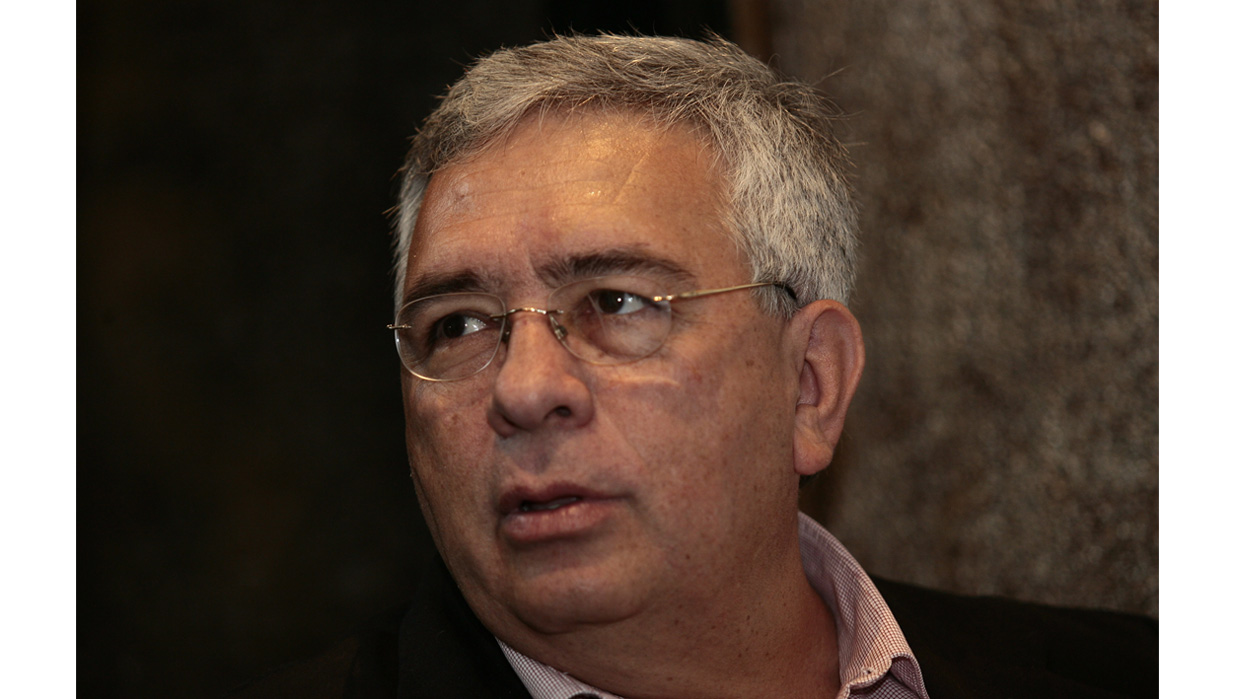
\includegraphics[width=300px]{EU_34515.jpg}%
\newline%
%
Por la corrupción del lenguaje empiezan otras formas de corrupción. Es una idea que viene  desde Andrés Bello para acá, utilizada por todas las ideologías políticas. El líder independentista, cuando surgieron las jóvenes repúblicas hispanoamericanas, decía que después haría falta la educación para construir la ciudadanía republicana, ya que,  según él, las palabras, expresiones y formas que utilizamos para comunicarnos ponen al descubierto, a veces inconscientemente, nuestros más profundos anhelos y temores; esperanzas y desilusiones, así como también, simpatías y antipatías.%
\newline%
%
Por mucho que controlemos nuestras emociones, al final nuestro lenguaje termina por sacar a la luz todo lo que llevamos por dentro. Por eso, una forma de conocer a las personas es observándolas como hablan.  El verbo no miente. Según Tucídides, en una de las primeras guerras civiles que se desencadenaron en el mundo griego, la de Córcira en el año 427 a. C., se llegó a tal extremo que hasta el idioma fue corrompido. Así, las conspiraciones eran presentadas como legítima autodefensa; la prudencia como cobardía. La violencia frenética como hombría y la moderación como falta de virilidad.%
\newline%
%
Mi padre, lector impenitente y político desde su juventud, me dijo en una oportunidad, que a los sistemas políticos aprendemos a reconocerlos por sus expresiones. El vocabulario, que de alguna forma institucionaliza un sistema político,  dice mucho de las corrientes subterráneas que lo alimentan. El general macedonio,  Pérdicas, decía: “los regímenes políticos  tiene cada uno su lengua como si se tratara de seres vivos. Un lenguaje tiene la democracia, otro la oligarquía, también existe uno para la tiranía y otro para la monarquía”.%
\newline%
%
Uno de los testimonios más impresionantes al respecto lo ofrece el escritor judío alemán, Víctor Klemperer, quien se negó a renunciar a alguna de estas dos nacionalidades, en plena barbarie del nacionalismo étnico y totalitario. Él sobrevivió a la persecución anotando en su diario durante 13 años los términos capitales de La Lengua del Tercer Reich.  Pudo así constatar que las mentiras y el salvajismo totalitario son fenómenos íntimamente ligados a la corrupción del dialecto.%
\newline%
%
Klemperer pudo mostrar con claridad cómo el nazismo impuso su dominación no solo mediante la Gestapo y los campos de concentración, sino también manipulando el lenguaje, logrando inocular, a través de él, su veneno totalitario. La Lengua del Tercer Reich era una obra para entender como los tiranos manipulan y pervierten este elemento. El escritor descubrió que la velada ponzoña inserta en el habla nazi era producto de su formación filológica, pero también de un hombre culto que identificó la importancia de las palabras para justificar y encubrir el horror.%
\newline%
%
La “corrupción del lenguaje”, como arbitrario e interesado cambio del sentido y significado de las palabras para adaptarlo a la ideología reaccionaria y oscura de algunas elites políticas, desde hace tiempo, inunda los medios de comunicación del mundo, sobre todo, en regímenes autocráticos.  La novela 1984 de George Orwell, es un vívido ejemplo, el Ministerio de la Verdad  se presenta como una institución encargada de administrar la verdad, aunque su principal función es su reescritura y falseamiento.%
\newline%
%
En la obra 1984, la “verdad” se entiende en el sentido de declaraciones como “La guerra es la paz”, “la libertad es esclavitud” y “la ignorancia es fuerza”. Orwell pretendió mostrar al mundo, el horror que supone el qué un Estado controle todo: El Gran Hermano. No hay vida privada, todo es público y todo se manipula a favor del partido único. “1984” tiene esa finalidad: llevar hasta el extremo la idea de Estado totalitario para alertar al ciudadano sobre los peligros que esto entrañaría.%
\newline%
%
En la novela de Orwell, esta alteración no solo se aplicaba a los periódicos, sino también a los libros, revistas, folletos, carteles, programas, películas, bandas sonoras, historietas para niños, entre otros. Diariamente y casi minuto por minuto, el pasado era puesto al día. “El que controla el pasado controla también el futuro” propugnaba el slogan del Partido en1984.  En muchos casos, como en el mundo de Orwell, si todos aceptan la mentira que impone el partido, si todos los testimonios dicen lo mismo, entonces la mentira pasará a la Historia y se convertirá en verdad.%
\newline%
%
Coordinador Nacional del Movimiento Político GENTE%
\newline%
%
Noelalvarez10@gmail.com%
\newline%
%
\end{document}